\documentclass[prl,aps,superscriptaddress,twocolumn,10pt,nolongbibliography]{revtex4-2}
\usepackage[pdftex]{graphicx}
\usepackage{color}
\usepackage{amsmath,amsthm,amssymb,mathtools}
\usepackage[colorlinks=true,allcolors=blue]{hyperref}
\usepackage{enumerate}
\usepackage{sidecap}
\sidecaptionvpos{figure}{c}
\usepackage{soul}

% for inline codes
\usepackage{listings}
\usepackage{color}
\definecolor{codegreen}{rgb}{0,0.6,0}
\definecolor{codegray}{rgb}{0.5,0.5,0.5}
\definecolor{codepurple}{rgb}{0.58,0,0.82}
\definecolor{backcolour}{rgb}{0.95,0.95,0.92}
\lstdefinestyle{mystyle}{
    backgroundcolor=\color{backcolour},
    commentstyle=\color{codegreen},
    keywordstyle=\color{magenta},
    numberstyle=\tiny\color{codegray},
    stringstyle=\color{codepurple},
    basicstyle=\footnotesize,
    breakatwhitespace=false,
    breaklines=true,
    captionpos=b,
    keepspaces=true,
    numbers=left,
    numbersep=5pt,
    showspaces=false,
    showstringspaces=false,
    showtabs=false,
    tabsize=2
}
\lstset{style=mystyle}

\newcommand{\notes}[1]{\textbf{\textcolor[rgb]{1,0,0.5}{#1}}}
\newcommand{\mick}[1]{\textbf{\textcolor[rgb]{0,0.6,0.3}{#1}}}

\begin{document}
\title{CS 412: Project Proposal for Microbusiness Density Forecasting}
\author{Kittithat Krongchon (krongch2)}
\affiliation{Department of Physics, University of Illinois at Urbana-Champaign}
\author{Ting Cheng (tingc4)}
\affiliation{Gies College of Business, University of Illinois at Urbana-Champaign}
\date{\today}

\maketitle

% Briefly introduce your task in the selected challenge. What is the input and what is the output?
% Getting to know your data. How large is it? What is the type of your data (categorical, numerical, etc)? 
% Are there any network, text or image data included?
\section{Introduction}
\begin{figure}
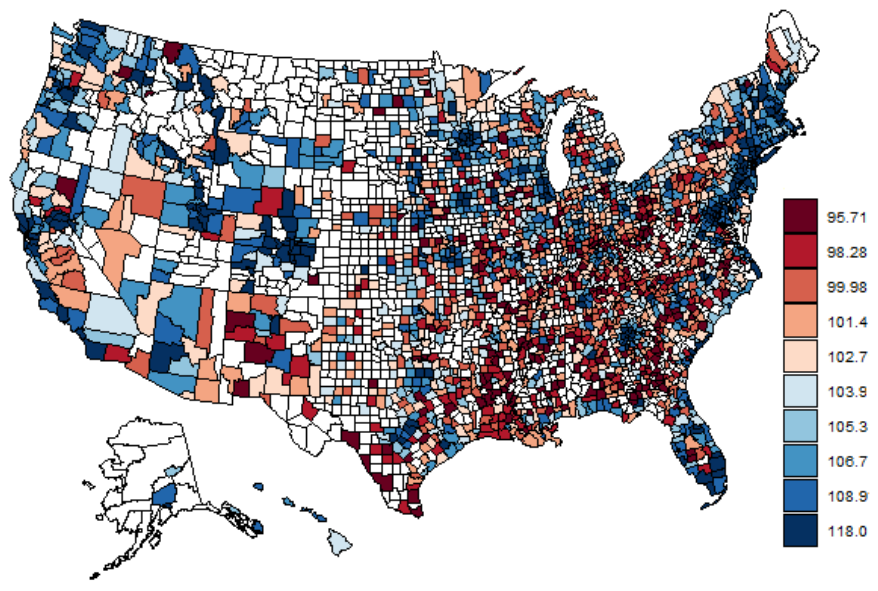
\includegraphics[width=3in]{figs/activity.png}
\caption{\label{fig:activity}
Microbusiness activity index by county in December 2021.
}
\end{figure}

Policymakers in the United States attempt to create economies that are robust to industry downturns. 
The success (or limitation) of new policies heavily relies on the data of business entities. 
Gaining accurate visibility into enabling economic decisions, however, is a challenging task because a large number of ``microbusinesses'', defined as businesses with ten or fewer employees, are often too small or too new to be included in standard data sources.
To overcome this challenge, the Venture Forward team at GoDaddy has studied tens of millions of microbusinesses in the United States for several years and has made the survey data publicly available. 
Thus, using data science techniques will enable policy leaders to gain more insights, which will be helpful for microbusiness entrepreneurs. 
This competition serves as a platform for participants to broaden the vision on the economic impact. 

\section{Data interpretation}
The task for this competition is to forecast microbusiness activity (Fig.~\ref{fig:activity}) across the United States, as measured by the density of microbusinesses for each of the 3142 counties~\cite{yu2021godaddy}.
The values for this column are provided on a monthly basis, starting from August 1, 2019 to October 1, 2022. 
The participants are predicting the microbusiness density for the next month. 
Thus, the total number of given records is $3142 \times 39 = 122538$ rows of data.
The other columns that are provided include the percentage of households in the county with access to broadband of any type, the percent of the population in the county over age 25 with a 4-year college degree, the percent of the population in the county born outside of the United States, the percent of the workforce in the county employed in information related industries, and the median household income in the county. 
These extra columns serve as features in training models.
The total size of these datasets is 10.93MB and all of them are numerical data without unstructured data. 

In this proposal, we will explore several training approaches, most of which can be put into two classes, namely auto-regressive models and tree-based models. 

% How do you plan to solve it? Explain your idea at a high-level. (You may revise it or even propose a completely new one later. We just need to know that you have already spent some time thinking about it.)
% List at least 2 baseline approaches you would like to compare with. Add citations if they are from research papers.
\section{Method}
For a time-series data, the auto-regressive integrated moving average (ARIMA) model is a widely used model that is based on constructing a model that depends on values at a different time. 
This type of model depends on the values of variables in the past, which is given by 
\begin{align}
y_t - \alpha_1 y_{t-1} &\cdots - \alpha_p y_{t-p} \nonumber \\
&= \epsilon_t + \theta_1 \epsilon_{t-1} + \cdots + \theta_q \epsilon_{t-q},
\end{align}
where $p$ and $q$ denote the order of time lags of the data (called the autoregressive model) and errors (the moving-average model). 
This model can be generalized to include the multiplicity of the roots as given by 
\begin{align}
(1 - \sum_i^p \alpha_i L^i) (1 - L)^d y_t = (1 + \sum_i^q \theta_i L^i) \epsilon_t,
\end{align}
where $L$ is the lag operator, which moves the data by one unit of time, and $d$ is the multiplicity. 
We solve this model by looping through different combinations of $(p, d, q)$ to find the model that yields the lowest Akaike information criterion (AIC) value. 
In our analysis, the model called seasonal-ARIMAX (SARIMAX) is used, which is an extension to the ARIMA model to capture seasonal data with exogenous variables.

Another class of techniques to be explored is tree-based models, such as random forest and XGBoost~\cite{chen2016xgboost}.
Random forest is a prediction algorithm, which is an extension of a decision tree. 
The algorithm works as follows. First, we perform a random selection with replacement on the data, i.e. bootstrapping. 
Then, we generate a decision tree on a randomly selected subset of feature variables. 
Once all the decision trees (hence forest) are obtained, we use them to predict the dependent variable from a given sample set of feature variables.
For the evaluation of our answers, we will use symmetric mean absolute percentage error (SMAPE) and root-mean-square error (RMSE).

% A timeline that specifies your plan to finish the course project.
\section{Timeline}
Our analysis involves two milestones. 
First, the training of time-series data without exogenous variables should be completed, which will be our baseline for a simple solution. 
Next, the density data will be trained with the seasonal information and exogenous variables included. 
We expect to arrive at this stage by March 15, 2023.

After the auto-regressive models are well explored, we will move on to the tree-based models. 
We expect to complete the training models using random forest and XGBoost by April 15, 2023. 

% Argue on the feasibility to finish the task on the selected challenge. 
% If your framework is too complicated, you might struggle to implement it. 
% Feel free to use existing tools and packages (e.g., repositories on GitHub).
\section{Feasibility}
Since the time-series prediction involved in this competition has been well explored in literature, and the existing tools are robust, this specific challenge has a straightforward workflow. 
The challenge for us, therefore, comes down to turning the provided information into an object that is suitable for each specific tool as discussed in the previous section.

\bibliography{paper}{}
\end{document}
